\chapter{Resultados}\label{chapter:results}

En este cap\'itulo se presentan los hallazgos clave del  análisis, enfoc\'andose en los resultados relativos a la relación entre el per\'iodo preferido y la excentricidad en diferentes áreas visuales, así como su relevancia en la lateralización hemisférica.

\section{Análisis de la relación entre el tamaño de los pRF y la excentricidad}

\begin{figure}[h]
	\centering
	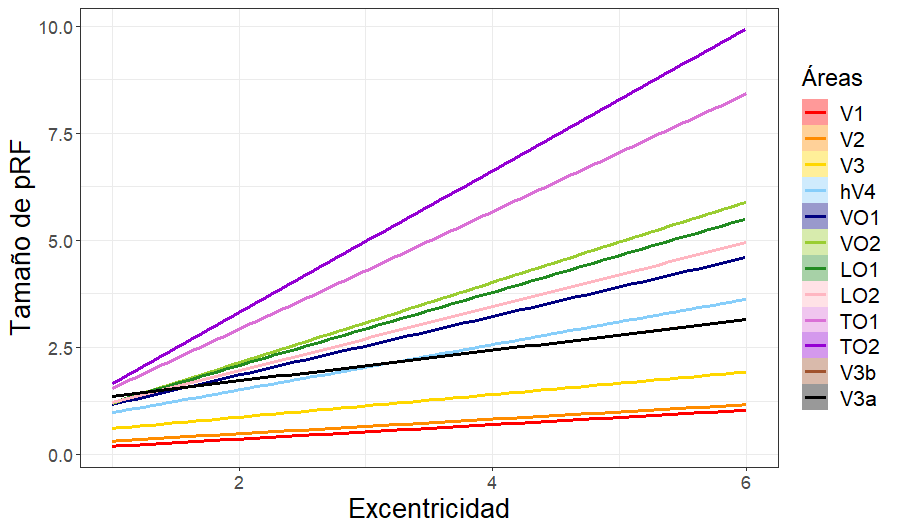
\includegraphics[scale=0.6]{Graphics/size_vs_eccen_bayesian}
	\caption{Gráfico que representa la relación entre el tama\~no de pRF y la excentricidad en las diferentes áreas visuales analizadas.}
	\label{fig:sigma_vs_eccen}
\end{figure}

Se llevó a cabo un análisis para examinar la relación entre el tamaño del pRF y la excentricidad en el campo visual, aunque no constituye el enfoque principal de este estudio. En la Figura \ref{fig:sigma_vs_eccen}, presentamos las rectas de regresión correspondientes a la relaci\'on entre estas variables. Observamos que el tamaño del pRF tiende a incrementar con la excentricidad, una tendencia que se manifiesta consistentemente a través de las diferentes áreas examinadas. De manera notable, la pendiente de estas rectas de regresión muestra un aumento progresivo al pasar de áreas visuales tempranas, como V1-V3, a áreas de procesamiento visual de nivel superior, como TO1. Este hallazgo está en consonancia con investigaciones previas [\cite{wandell_computational_2015}] y refuerza la comprensión de que el tamaño del pRF se expande con la complejidad funcional y jerárquica de las áreas visuales.

\section{Análisis de la relación entre el período preferido y la excentricidad}

En la figura \ref{fig:pp_vs_eccen}, se puede observar que en la mayoría de las áreas visuales analizadas, se cumplen los supuestos de que el período preferido tiende a aumentar con la excentricidad. Sin embargo, es importante destacar que existen variaciones en este patrón.

\begin{figure}[h]
	\centering
	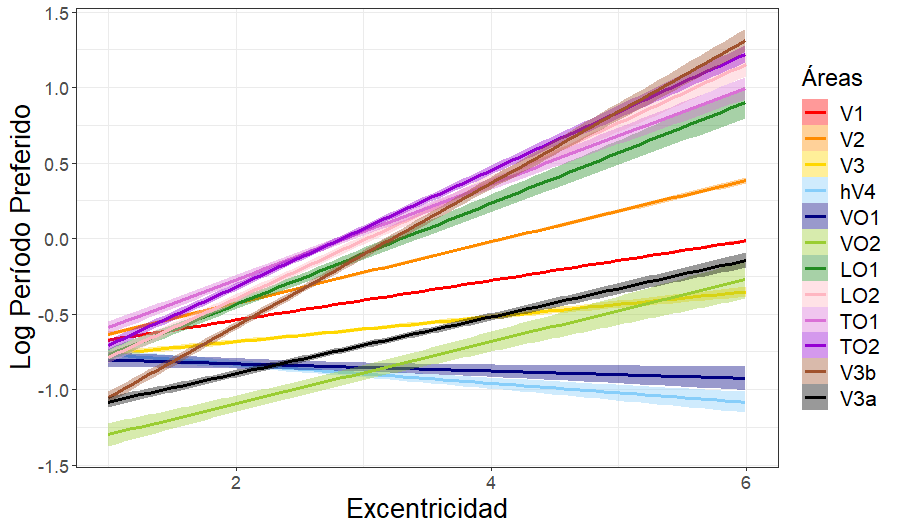
\includegraphics[scale=0.6]{Graphics/pp_vs_eccen}
	\caption{Gráfico que representa la relación entre el logar\'itmo del per\'iodo preferido de los v\'oxeles y la excentricidad, en las 12 áreas visuales analizadas.}
	\label{fig:pp_vs_eccen}
\end{figure}

En áreas visuales como hV4 y VO1, se observa una pendiente de crecimiento negativa. Este hallazgo sugiere que, a medida que la excentricidad aumenta, el período preferido tiende a disminuir. Este comportamiento atípico resalta la diversidad de respuestas visuales en diferentes regiones corticales.

Además, en áreas visuales superiores como LO1, LO2, TO1 y TO2,  se evidencia un aumento de la pendiente del período preferido con respecto a la excentricidad, comparado con las áreas visuales tempranas. Esta observación indica que estas áreas específicas muestran un patrón consistente de incremento en el período preferido a medida que se alejan del punto central de la visión, un aspecto que no se había abordado en ningún estudio previo que hayamos revisado.

Este análisis proporciona una comprensión más completa de cómo la excentricidad puede modular el período preferido en diversas áreas visuales, destacando la heterogeneidad funcional en la corteza visual.


\section{Resultados del modelo lineal mixto para el per\'iodo preferido en función de excentricidad y hemisferio}

\begin{table}[h]
	\centering
	\resizebox{\textwidth}{!}{
	\begin{tabular}{@{}lcccccccccccc@{}}
		\toprule
		 & \multicolumn{4}{c}{\large \textbf{Excentricidad}} & \multicolumn{4}{c}{\large \textbf{Hemisferio}} & \multicolumn{4}{c}{\large \textbf{Excentricidad:Hemisferio}} \\
		\midrule
		\large \textbf{Áreas} & \textit{Coef} & \textit{SE} & \textit{t-val} & \textit{BF10} & \textit{Coef} & \textit{SE} & \textit{t-val} & \textit{BF10} & \textit{Coef} & \textit{SE} & \textit{t-val} & \textit{BF10} \\
		\midrule
		V1 & 0.147 & 0.002 & 67.939 & 8.32e+256 & 0.097 & 0.011 & 8.960 & 9.78e-04 & -0.033 & 0.003 & -10.939 & 2.01e+21 \\
		V2 & 0.202 & 0.004 & 49.131 & 8.32e+256 & -0.034 & 0.019 & -1.753 & 1.47e+18 & -0.017 & 0.006 & -2.882 & 0.003 \\
		V3 & 0.134 & 0.006 & 20.973 & 1.06e+60 & 0.363 & 0.028 & 12.985 & 3.300 & -0.112 & 0.009 & -12.255 & 3.30e+28 \\
		hV4 & -0.033 & 0.014 & -2.322 & 9.71e+08 & 0.501 & 0.051 & 9.808 & 1.37e+35 & -0.076 & 0.018 & -4.088 & 1.210 \\
		VO1 & 0.015 & 0.016 & 0.943 & 4.66e-04 & 0.773 & 0.069 & 11.279 & 1.89e+63 & -0.096 & 0.022 & -4.273 & 3.710 \\
		VO2 & 0.218 & 0.027 & 8.155 & 7.53e+22 & -0.071 & 0.107 & -0.659 & 0.437 & -0.036 & 0.036 & -0.998 & 0.002 \\
		LO1 & 0.377 & 0.019 & 19.618 & 2.19e+109 & 0.452 & 0.061 & 7.442 & 4.350 & -0.152 & 0.025 & -6.152 & 7.96e+04 \\
		LO2 & 0.353 & 0.017 & 21.095 & 8.32e+256 & -0.362 & 0.060 & -6.071 & 2.01e+13 & 0.049 & 0.022 & 2.249 & 0.006 \\
		TO1 & 0.333 & 0.013 & 26.040 & 1.00e+208 & 0.069 & 0.058 & 1.190 & 0.008 & -0.050 & 0.020 & -2.548 & 0.013 \\
		TO2 & 0.398 & 0.010 & 39.021 & 8.32e+256 & 0.221 & 0.050 & 4.384 & 465.000 & -0.037 & 0.017 & -2.225 & 0.004 \\
		V3b & 0.502 & 0.015 & 34.160 & 8.32e+256 & 0.383 & 0.055 & 6.958 & 2.42e+23 & -0.039 & 0.020 & -1.966 & 0.003 \\
		V3a & 0.230 & 0.011 & 21.320 & 4.42e+158 & 0.126 & 0.047 & 2.703 & 0.003 & -0.059 & 0.014 & -4.063 & 0.658 \\
		\bottomrule
	\end{tabular}
	\caption{Tabla que resume los resultados del modelo lineal mixto \ref{mlm_pp} empleado para analizar el per\'iodo preferido de los v\'oxeles en diferentes áreas visuales. Cada fila representa los resultados del modelo para una área visual específica. Para cada variable fija del modelo, la tabla muestra la estimación del coeficiente (Coef), el error estándar (SE) y el valor t (t-val). Además, se incluye el factor de Bayes (BF10) de la comparación entre modelos. El BF10 en la columna Excentricidad corresponde a la comparación entre el modelo \ref{m_1} y \ref{m_2}; en la columna Hemisferio, se refiere a la comparación entre el modelo \ref{m_2} y \ref{m_3}; y en la columna Excentricidad:Hemisferio, a la comparación entre los modelos \ref{m_3} y \ref{mlm_pp}.}
	\label{tab:mlm_results_pp}
}
\end{table}

En esta secci\'on, se aborda el núcleo central de esta tesis: el análisis del impacto de la frecuencia espacial sobre los hemisferios cerebrales. 

En el modelo \ref{mlm_pp}, la variable de interés es el per\'iodo preferido, que representa el inverso de la frecuencia espacial. En este modelo, se busca explicar la relación entre el per\'iodo preferido y dos variables independientes: la excentricidad y el hemisferio. Además, se incorporan las diferencias entre sujetos y estímulos para obtener un entendimiento más completo de los factores que influyen en el mismo.

Los resultados obtenidos de dicho modelo, se detallan en la Tabla \ref{tab:mlm_results_pp}. En esta tabla, las filas ilustran las diferentes áreas visuales analizadas mediante el modelo \ref{mlm_pp}, mientras que las columnas, excepto la primera (\'Areas), representan las variables fijas con sus respectivos resultados:  estimación de los coeficientes (Coef), error estándar (SE) y t-valor (t-val). Adicionalmente, se insert\'o una columna con el factor de Bayes (BF10) resultante de la comparaci\'on de cada uno de los modelos propuestos en la secci\'on \ref{mlm}. El BF10 contenido en la columna Excentricidad es resultado de la comparaci\'on del modelo nulo (\ref{m_1}) con el modelo con excentricidad (\ref{m_2}). En la columna Hemisferio de la tabla, se muestra el BF10 de la comparaci\'on del modelos con excentricidad  y el modelo aditivo con excentricidad y hemisferio (\ref{m_3}). En la \'ultima columna se observa el BF10 del modelo aditivo comparado con el modelo con interacci\'on de excentricidad y hemisferio (\ref{mlm_pp}).


%\begin{figure}
%	\centering
%	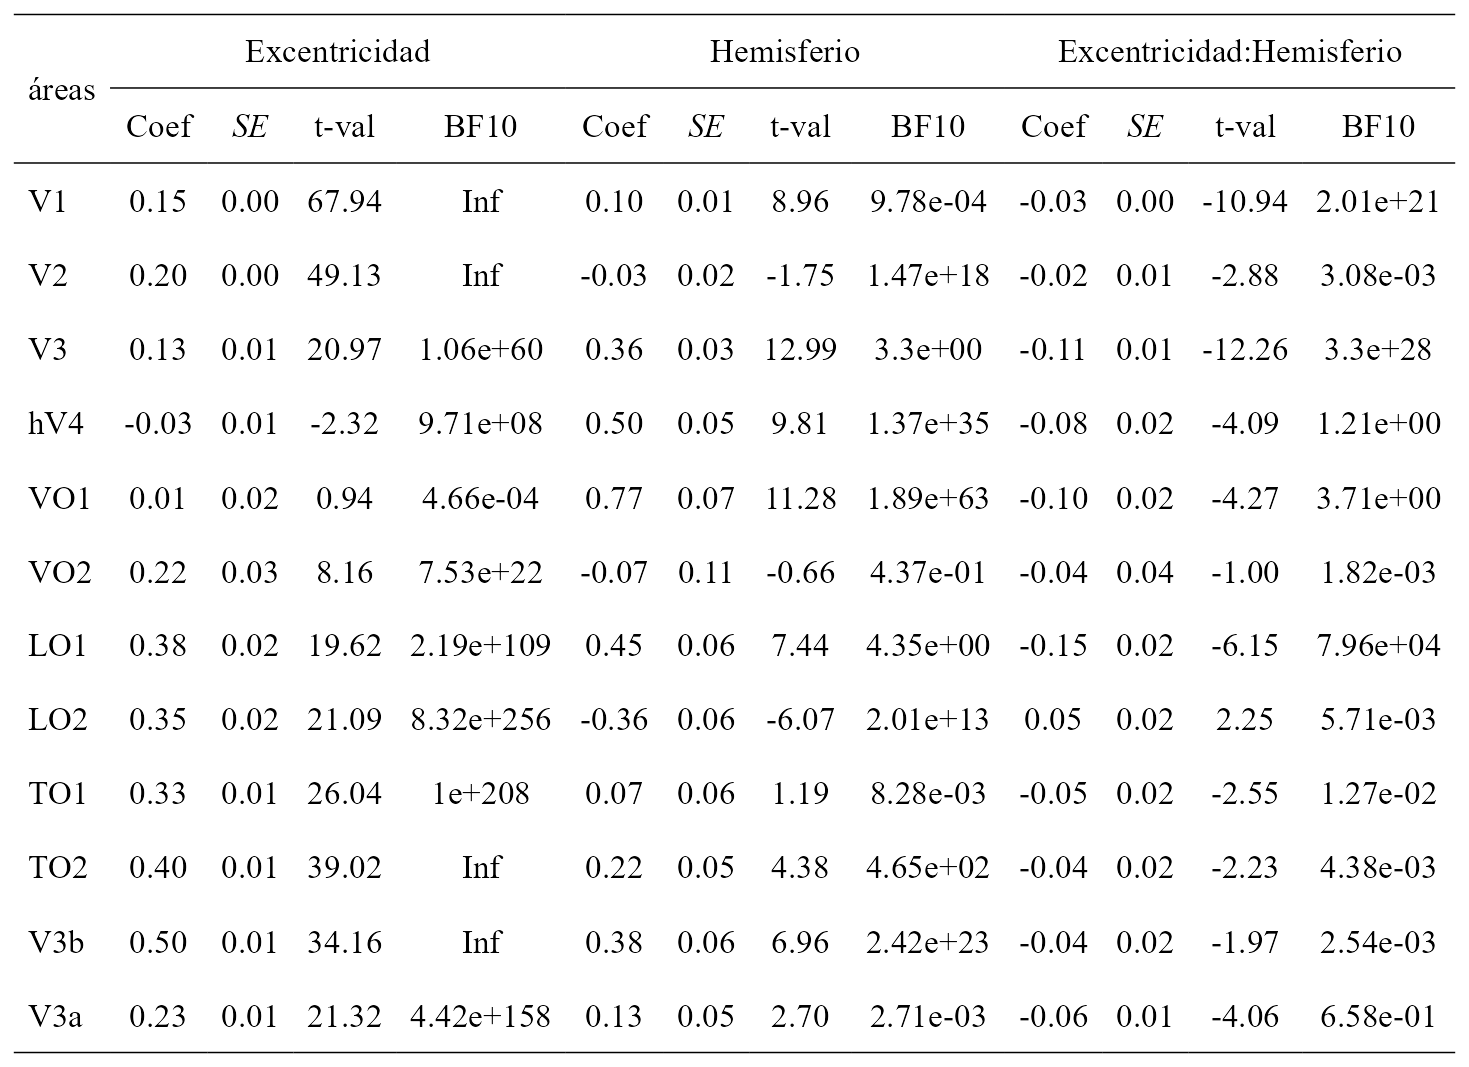
\includegraphics[scale=0.8]{Graphics/table_pp}
%	\caption{Tabla que resume los resultados del modelo lineal mixto \ref{mlm_pp} empleado para analizar el per\'iodo preferido de los v\'oxeles en diferentes áreas visuales. Cada fila representa los resultados del modelo para una área visual específica. Para cada variable fija del modelo, la tabla muestra la estimación del coeficiente (Coef), el error estándar (SE) y el valor t (t-val). Además, se incluye el factor de Bayes (BF10) para la comparación entre modelos. El BF10 en la columna 'Excentricidad' corresponde a la comparación entre el modelo \ref{m_1} y \ref{m_2}; en la columna 'Hemisferio', se refiere a la comparación entre el modelo \ref{m_2} y \ref{m_3}; y en la columna 'Excentricidad:Hemisferio', a la comparación entre los modelos \ref{m_3} y \ref{mlm_pp}.}
%	\label{fig:mlm_results_pp}
%\end{figure}



En la Tabla \ref{tab:mlm_results_pp}, se aprecia que, con excepción de hV4 y VO1, el tamaño del efecto de la excentricidad (Ver Tabla \ref{tab:mlm_results_pp}, columna Excentricidad) es relativamente grande, lo cual indica un aumento en el per\'iodo preferido con la excentricidad. Este hallazgo es respaldado tanto por el t-valor como por el factor de Bayes. Además, se observa un patrón consistente de incremento en la magnitud del efecto al pasar de áreas tempranas a aquellas de orden superior, corroborando lo evidenciado en la Figura \ref{fig:pp_vs_eccen}. En el caso de hV4, el coeficiente exhibe un signo negativo y una magnitud inferior en comparación con otras áreas, y es estadísticamente significativo según la prueba t de Student y el factor de Bayes. Respecto a V01, su coeficiente es notablemente pequeño, y ninguna de las pruebas mencionadas evidencia significancia.

\begin{figure}[h]
	\centering
	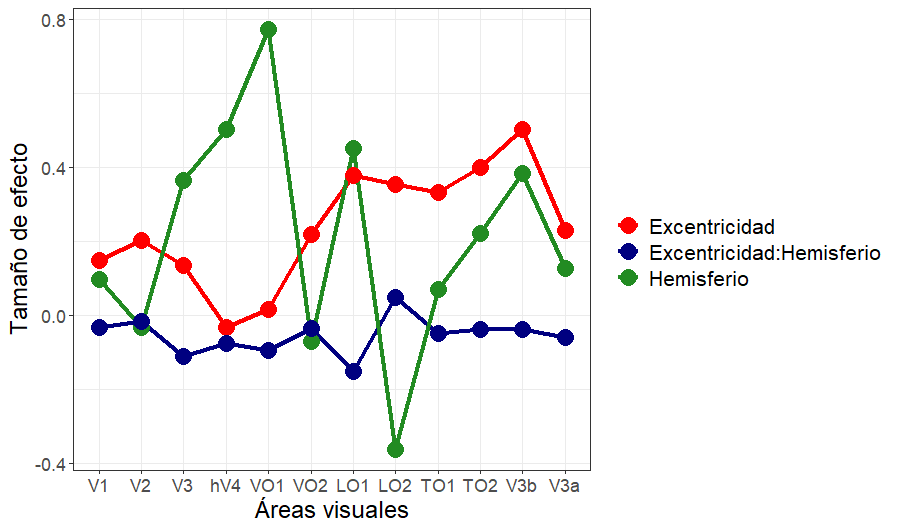
\includegraphics[scale=0.6]{Graphics/effect_size_coef_pp}
	\caption{Representación gráfica de los coeficientes estimados para las variables fijas del modelo lineal mixto \ref{mlm_pp}.}
	\label{fig:coeff}
\end{figure}

Resulta notable que hay un efecto de hemisferio (Ver Tabla \ref{tab:mlm_results_pp}, columna Hemisferio) significativo en casi todas las áreas con excepción de V02, pero con coeficientes pequeños en V1, V2, TO1, y V3a . En contraste, la mayor\'ia de las \'areas restantes (V3, hV4, VO1, LO1, TO2, V3b), presentan coeficientes relativamente grandes (Figura \ref{fig:coeff}), lo cual indica que  el per\'iodo preferido de los v\'ertices corticales en el hemisferio derecho es significativamente mayor que en el izquierdo. Al graficar (Ver Figura \ref{fig:hem}) la relaci\'on entre el per\'iodo preferido y la excentricidad de todas las \'areas visuales analizadas, se pudo observar que esta diferencia es m\'as pronunciada en las \'areas hV4 y VO1. 

Las interacciones entre excentricidad y hemisferio (Ver Tabla \ref{tab:mlm_results_pp}, columna Excentricidad:Hemisferio), fueron significativas en varias áreas, pero su magnitud fue relativamente baja en todas las regiones analizadas.

\begin{figure}[h]
	\centering
	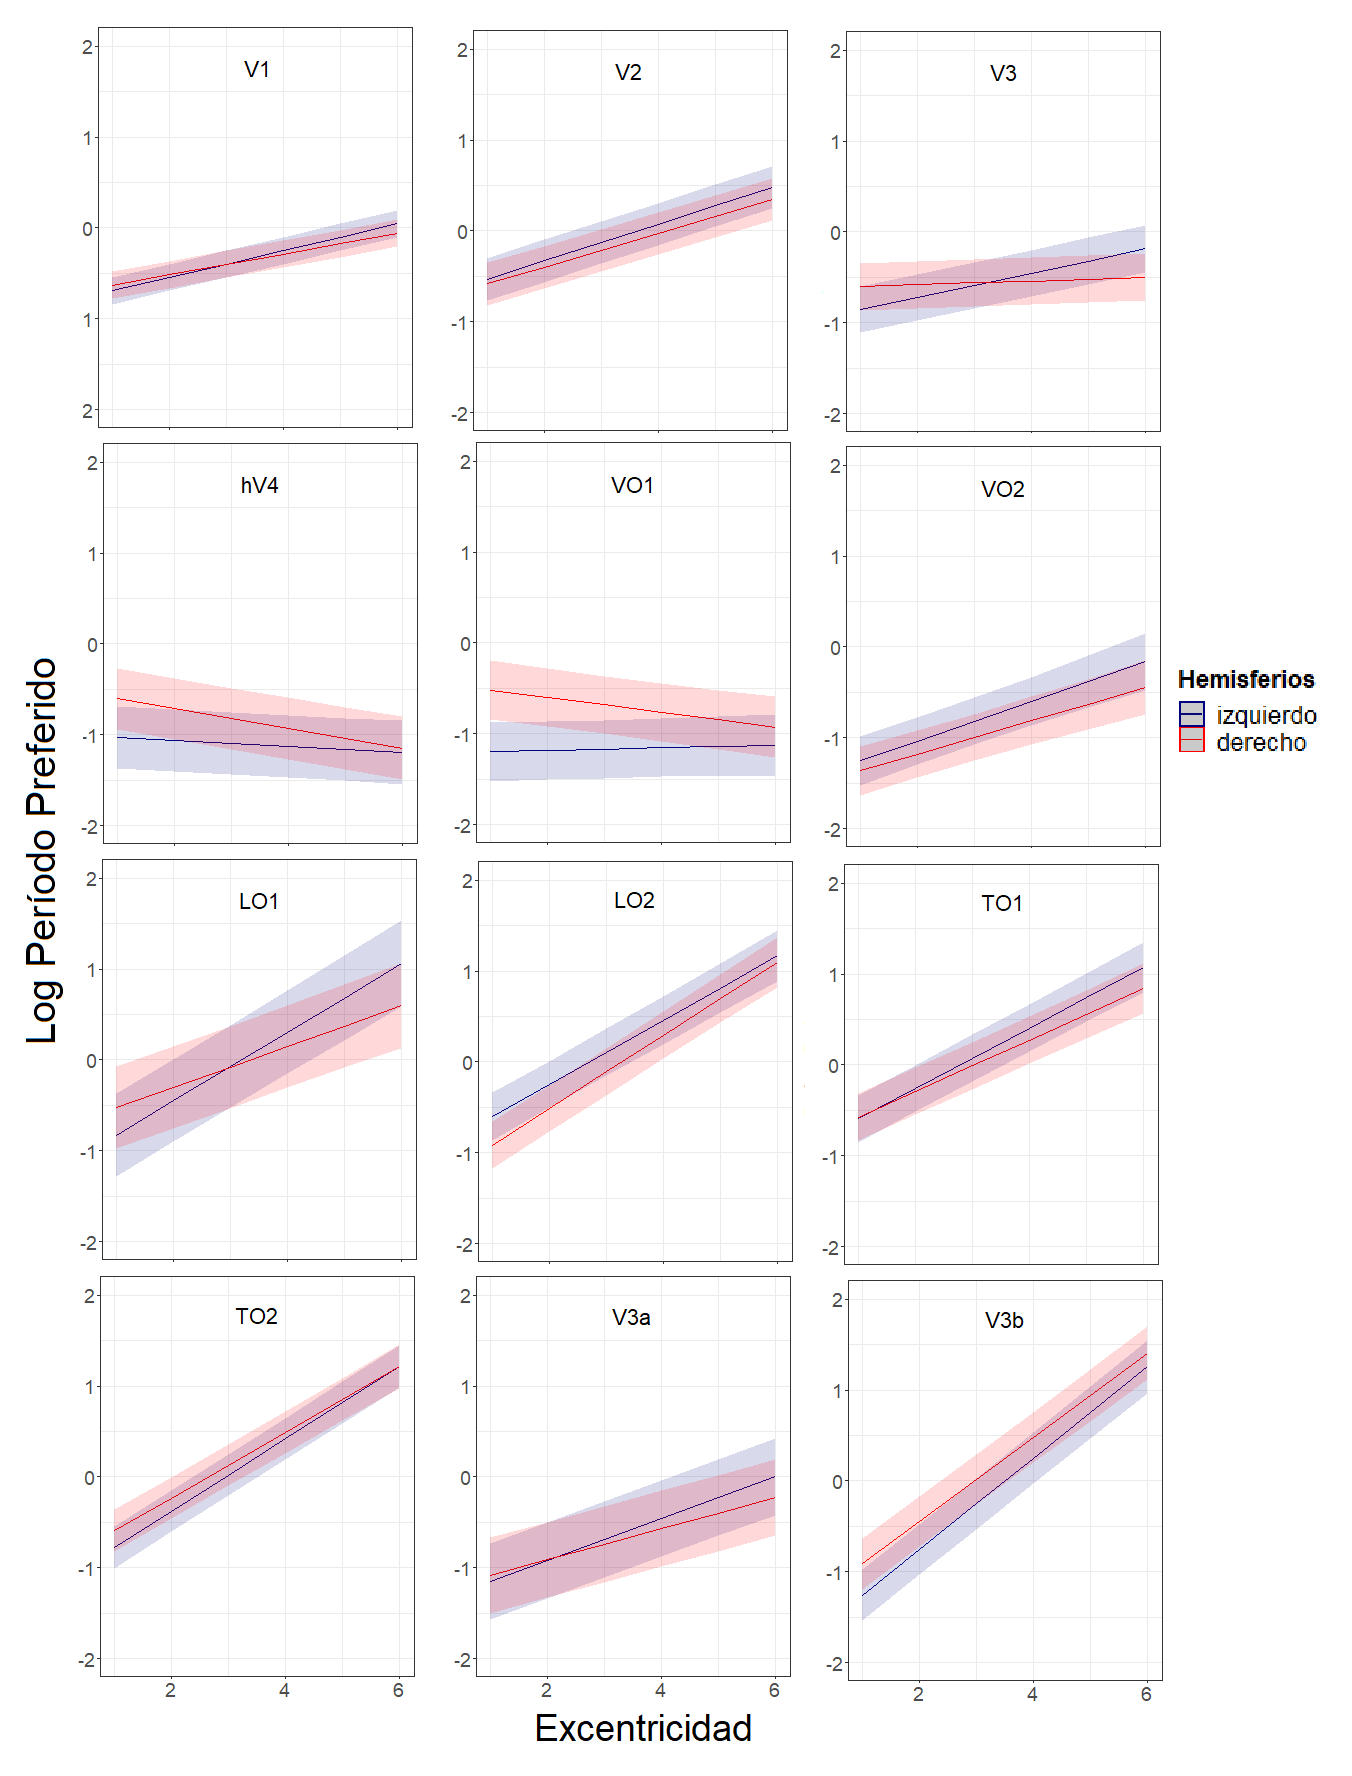
\includegraphics[scale=0.5]{Graphics/compuesto_rois_pp_vs_eccen_hem}
	\caption{Conjunto de gráficas representando la relación entre el logaritmo del per\'iodo preferido de los v\'oxeles y la excentricidad en los dos hemisferios cerebrales, para las 12 áreas visuales analizadas.}
	\label{fig:hem}
\end{figure}













